% !TEX program = xelatex
% !BIB program = bibtex
\documentclass[11pt, openright, twoside]{report}
\usepackage[english,portuguese]{babel}

\selectlanguage{english}

%% %%%%%%%%%%%%%%%%%%%%%%%%%%%%%%%%%%%%%%%%%%%%%%%%%%%%%%%%%%%%%%%%%%%%%%%%%%%%
%% %%%%%%%%%%%%%%%%%%%% IMPORTANT: SET THE INFORMATION %%%%%%%%%%%%%%%%%%%%%%%%
%% %%%%%%%%%%%%%%%%%%%%%%%%%%%%%%%%%%%%%%%%%%%%%%%%%%%%%%%%%%%%%%%%%%%%%%%%%%%%
\newcommand{\departmentname}{INFORMÁTICA}
\newcommand{\thesisname}{Formalization and Runtime Verification of Invariants for Robotic Systems}
\newcommand{\studentname}{Ricardo Jorge Dias Cordeiro}
\newcommand{\coursename}{Engenharia Informática}
\newcommand{\specname}{Especialização em Interação e Conhecimento}
%\newcommand{\versaoprovisoria}{Versão Provisória} % TODO: Blank for final version
\newcommand{\thesistype}{Dissertação}
\newcommand{\alcides}{Prof. Doutor Alcides Miguel Cachulo Aguiar Fonseca}
\newcommand{\chris}{Prof. Doutor Christopher Steven Timperley}
%% %%%%%%%%%%%%%%%%%%%%%%%%%%%%%%%%%%%%%%%%%%%%%%%%%%%%%%%%%%%%%%%%%%%%%%%%%%%

% -----------------------------------------------------------------------------
% Packages defined by the student
%% %%%%%%%%%%%%%%%%%%%%%%%%%%%%%%%%%%%%%%%%%%%%%%%%%%%%%%%%%%%%%%%%%%%%%%%%%%%
%% Important packages
\usepackage{times}
\usepackage{graphicx}
\usepackage{subcaption}

\usepackage{csquotes}
\usepackage{makeidx}

% Packages for the cover
\usepackage{fontspec}
\newfontfamily{\coverfont}{arial-narrow}
    [Path = ./assets/, 
    Extension = .ttf, 
    UprightFont = *-regular,
    BoldFont = *-bold
    ]
\usepackage{anyfontsize}
\usepackage{afterpage}

\usepackage{changepage}

% Positioning
\usepackage{float}

% Page format
\usepackage[dvips]{geometry}
\geometry{
    a4paper=true,
    portrait=true,
    left=2.5cm,
    right=2.5cm,
    top=2.5cm,
    bottom=2.5cm
}

%% %%%%%%%%%%%%%%%%%%%%%%%%%%%%%%%%%%%%%%%%%%%%%%%%%%%%%%%%%%%%%%%%%%%%%%%%%%%%
%% Other required packages

% Bibliography
\bibliographystyle{plainnat}
\usepackage[numbers]{natbib}

% Math
\usepackage{amsmath}
\usepackage{amssymb} 
\usepackage{amsthm}

% Images
\usepackage{color}
\usepackage[table, xcdraw,dvipsnames]{xcolor}

% Code listings
\usepackage{caption} 
\usepackage{listings}

% Text and pdf
\usepackage{pdfpages}
\usepackage{xspace}
\usepackage[shortlabels]{enumitem}

% Links
\usepackage[colorlinks=true, citecolor=Blue]{hyperref}
\usepackage[all]{hypcap}
\usepackage{cleveref}

%BNF grammars
%\usepackage{simplebnf}


% Generated the pdf with information
\hypersetup{
    pdfauthor={\studentname},                                       
    pdftitle={\thesisname},                                         
    pdfsubject={\thesistype in \coursename},                        
    pdfkeywords={Keyword1, Keyword2, Keyword3, Keyword4}                 % TODO
}

%% %%%%%%%%%%%%%%%%%%%%%%%%%%%%%%%%%%%%%%%%%%%%%%%%%%%%%%%%%%%%%%%%%%%%%%%%%%%%
%% Other packages




%% %%%%%%%%%%%%%%%%%%%%%%%%%%%%%%%%%%%%%%%%%%%%%%%%%%%%%%%%%%%%%%%%%%%%%%%%%%%%
%% Auxiliary commands
\newcommand{\cleanpage}{\newpage\mbox{}\thispagestyle{empty}\newpage}

\newcommand{\startpagecounter}[1]{\setcounter{page}{1}\pagenumbering{#1}}

% Commands for TODOS
\newcommand{\nb}[2]{\fcolorbox{gray}{yellow}{\bfseries\sffamily\scriptsize#1}{\sf\small$\blacktriangleright$\textit{#2}$\blacktriangleleft$}}
\newcommand\todo[1]{\nb{Todo}{#1}}

\newcommand{\missref}{\fcolorbox{gray}{red}{\bfseries\sffamily\scriptsize\textcolor{white}{REF}}}


% -----------------------------------------------------------------------------

% Index
\makeindex

% -----------------------------------------------------------------------------
% Begin of the thesis
\begin{document}

\startpagecounter{roman}

% Cover
% !TeX root = ../main.tex
% %%%%%%%%%%%%%%%%%%%%%%%%%%%%%%%%%%%%%%%%%%%%%%%%%%%%%%%%%%%%%%%%%%%%%%%%%%%%%
% %%%%%%%%%%%%%%%%%%% Cover: No need to change anything here %%%%%%%%%%%%%%%%%% 
% %%%%%%%%%%%%%%%%%%%%%%%%%%%%%%%%%%%%%%%%%%%%%%%%%%%%%%%%%%%%%%%%%%%%%%%%%%%%%
\thispagestyle{empty}

% Sets the new page geometry
\newgeometry{
    left=3cm,
    right=3cm,
    top=1cm,
    bottom=0.4cm
}

% Set the cover font to Arial Narrow
{\coverfont

% Center the page text
\begin{center}

% Universidade de Lisboa, Faculdade de Ciências, Departamento de Informática
{\large 
UNIVERSIDADE DE LISBOA
\vspace{8.0pt}

FACULDADE DE CIÊNCIAS
\vspace{8.0pt}

DEPARTAMENTO DE \departmentname
\vspace{8.0pt}
}

\vspace{46pt}

% Ciências ULisboa Logo

\includegraphics{images/logotipo.png}

\vspace{117pt}

% Title of the thesis
{\fontsize{17}{19.55}\coverfont\textbf{\thesisname}}

\vspace{110pt}

% The student name
{\fontsize{15}{17.25}\coverfont\studentname}

\vspace{74pt}

% Designação do curso e especialidade
{\fontsize{13}{14.95}\coverfont\textbf{Mestrado em {\coursename}}

\vspace{0.65pt}

\specname
}

\vspace{22pt}

% Versão Provisória
{\fontsize{11}{12.65}\coverfont\versaoprovisoria}

\vspace{27pt}

% Supervisors
{\fontsize{13}{14.95}\coverfont
{\thesistype} orientad\ifthenelse{\equal{\thesistype}{Dissertação}}{a}{o} por: 

\firstadvisor

\vspace{3pt}

\secondadvisor

\vspace{3pt}

\thirdadvisor
}

~
\vfill

% Year the work was done
{\Large\the\year{}}

\end{center}
}

% Restore the page geometry
\restoregeometry
\cleanpage

% Acknowledgements
% !TeX root = ../main.tex
% %%%%%%%%%%%%%%%%%%%%%%%%%%%%%%%%%%%%%%%%%%%%%%%%%%%%%%%%%%%%%%%%%%%%%%%%%%%%%%
% Acknowledgements
\selectlanguage{english}

\pagestyle{plain}

\vspace*{2cm}
\begin{center}
\Large \bf Acknowledgments
\end{center}
\vspace*{1cm} \setlength{\baselineskip}{0.6cm}

I would like to thank my coordinator, Prof. Alcides Fonseca, for the exceptional way of teaching not only through the making of my thesis but also throughout all my academic courses. 

My coordinator Prof. Chris Timperley for taking his time to help me in this chapter of his life where he had to take care of his baby. 

My upperclassman Paulo and Catarina, for all the advice and help. 

All my friends who spent time with me know that somehow you helped me through this process. 

All my family, in particular my grandparents. 

My little brother. 

In the end, and more importantly, my mother for taking care of me all my life and giving me the opportunity to follow this path.

\cleardoublepage~\vfill

\begin{flushright}\textit{"Dreams breathe life into men, and can cage them in suffering. Men live and die by their dreams, but long after they've been abandoned, they still smolder deep in men's hearts. Some see nothing more than life and death. They are dead! For they have no dreams."}\end{flushright}
\begin{flushright}\textit{Kentaro Miura in Berserk}\end{flushright}

\selectlanguage{english}

\cleardoublepage 

% Resumo em Portugues
% !TeX root = ../main.tex
% %%%%%%%%%%%%%%%%%%%%%%%%%%%%%%%%%%%%%%%%%%%%%%%%%%%%%%%%%%%%%%%%%%%%%%%%%%%%%%
% Resumo em Português
\selectlanguage{portuguese}

\vspace*{2cm}
\begin{center} \Large \bf Resumo
\end{center}
\vspace*{1cm} \setlength{\baselineskip}{0.6cm}

A Robótica tem uma grande influência na sociedade atual, ao ponto que a falha em algum robô que seja crucial pode impactar o modo em como nós vivemos, se por exemplo um carro autônomo provocar a morte de algum passageiro devido a um defeito, futuros e atuais utilizadores deste modelo irão certamente ficar apreensivos em relação à sua utilização. Assegurar que robôs reproduzam um comportamento correto pode assim salvar bastante dinheiro em estragos ou até mesmo as nossas vidas.

As práticas atuais em relação à testagem de robôs são vastas e envolvem métodos como simulações, verificação de logs, ou testagem em campo, frequentemente, um denominador comum entre estas práticas é a necessidade de um humano pessoalmente analisar e determinar se o comportamento de um robô é o correto. A automatização deste tipo de análise poderia não só aliviar o trabalho de técnicos especializados, facilitando assim a realização de testes, mas também possivelmente detetar falhas no comportamento dos robôs que de outra maneira não seriam identificados devido a erros humanos.

Esta dissertação almeja explorar o problema da automatação na deteção de erros comportamentais em robôs num ambiente de simulação, introduzindo uma linguagem de domínio (DSL) direcionada a especificar as propriedades de robôs em relação ao seu ambiente, e a geração de software de monitorização capaz de detetar a transgressão destas propriedades.

A DSL necessita de expressar requisitos de determinados estados ou eventos durante a simulação, desta maneira precisa de apresentar determinadas características. Palavras-chave para representar relações temporais, como o robô "nunca", ou "eventualmente" o robô. Referências a estados anteriores, como a velocidade do robô é sempre maior que no estado anterior. Atalhos para se referir a certas utilidades, como "posição" ou "velocidade" do robô.

A DSL também assume que o robô irá ser executado por meio da framework ROS (Robot Operating System), que é amplamente usada na indústria da robótica. A arquitectura do ROS engloba características como publish-subscribe entre "tópicos" e tipos de mensagem, estas características são tidas em conta e foram integradas no desenvolvimento da DSL.

O software de monitorização gerado refere-se a um ficheiro python que correrá sobre a framework ROS. A geração deste ficheiro assume que a monitorização será feita no simulador Gazebo, isto porque para obter dados como a posição ou velocidade absoluta de um robô na simulação é necessário aceder a "tópicos" especificos que estão hardcoded. A geração de um ficheiro capaz de executar a monitorização significa que esta pode operar independente de um robô, ou seja, a automatização da monitorização pode ser realizada a respeito de um robô ou um grupo de robôs e o seu ambiente.

Resultados mostram que é possível expressar propriedades temporais e posicionais de robôs com ajuda da DSL, assim como automatizar a monitorização da violação de alguns comportamentos esperados do robô em relação ao seu estado ou certos eventos durante uma simulação.


*possiveis problemas, e futuro* - proof of language or that it works - better information on the errors - frequency of checking the properties can be modified in some circunstances to not check at every iteration - alargar a outros simuladores - integration with other tools liek scenario generation

%Para documentos em Português: Resumo em português até \textbf{300} palavras.
%Para documentos em língua estrangeira: Resumo em português entre \textbf{1200} e \textbf{1500} palavras.

\vfill

\begin{flushleft}
\textbf{Palavras-chave:}
Robótica, Linguagem de domínio, Deteção de erros, Automação, Monitorização
\end{flushleft}

\selectlanguage{english}
\cleardoublepage

% Abstract in English
% !TeX root = ../main.tex
% %%%%%%%%%%%%%%%%%%%%%%%%%%%%%%%%%%%%%%%%%%%%%%%%%%%%%%%%%%%%%%%%%%%%%%%%%%%%%%
% Abstract in English
\vspace*{2cm}
\begin{center}
\Large \bf Abstract
\end{center}
\vspace*{1cm} \setlength{\baselineskip}{0.6cm}

Robotics has a big influence in today's society, so much that a potential failure in a robot may have extraordinary costs, not only financial but can also cost lives.

Current practices in robot testing are vast and involve such methods as simulations, log checking, or field tests. The frequent common denominator between these practices is the need for human visualization to determine the correctness of a given behavior. Automating this analysis could not only relieve this burden from a high-skilled engineer but also allow for massive parallel executions of tests, that could potentially detect behavioral faults in the robotic system that would otherwise not be found due to human error or lack of time.

For my thesis, I have developed a domain-specific language to specify the properties of robotic systems in ROS. Specifications written by developers in this language can be compiled to a monitor ROS module, that will detect violations of those properties. I have used this language to express the temporal and positional properties of robots, and we have automated the monitoring of some behavioral violations of robots in relation to their state or events during a simulation.

*Evaluation ?*

\vfill

\begin{flushleft}
\textbf{Keywords:}
Robotics, Domain-specific language, Runtime Monitoring, Error detection, Automation
\end{flushleft}

\cleardoublepage

\pagestyle{plain}

% Table of Contents
\tableofcontents

% All the remaining lists
\listoffigures
\addcontentsline{toc}{chapter}{List of Figures}

\listoftables
\addcontentsline{toc}{chapter}{List of Tables}

\lstlistoflistings
\addcontentsline{toc}{chapter}{Listings}

\cleardoublepage

% ---------------------------------------------------------------------
% Thesis content
\startpagecounter{arabic}

% !TeX root = ../main.tex
% %%%%%%%%%%%%%%%%%%%%%%%%%%%%%%%%%%%%%%%%%%%%%%%%%%%%%%%%%%%%%%%%%%%%%%%%%%%%%%
% Introduction
\chapter{Introduction}
\label{chap:introduction}

This thesis aims to explore a possible solution for automation in the testing of robotic systems through a domain-specific language (DSL) and simulation-based monitoring software.

A DSL is a programming language that is written for a specific domain, it usually provides a higher level of abstraction and is simpler than other languages mainly because they are intended to be used by people knowledgeable of the domain.

This chapter intends to introduce the motivation for this work (\autoref{sec:motivation}), present the problem statements of such an approach (\autoref{sec:problem}), discuss the objectives (\autoref{sec:objectives}), show a motivational example of the developed work (\autoref{sec:motivationalexample}), present the expected contributions (\autoref{sec:contributions}), and finally summarize the structure of the rest of the document (\autoref{sec:structure}).


% ------------------------------------------------------------------------------
% Motivation
\section{Motivation}
\label{sec:motivation}

Robotics already significantly impact our current society, in industry, in medicine, in agriculture, or leisurely in sports contests or personal use. Robotics often take critical roles like the example of robot arms in car assembly lines or autonomous farms. The tendency is for robot usage to keep growing at a global level. 

Robotic Systems are non-deterministic, mainly because robots interact directly with the real world. Testing software in such environments is complex, as many variables can change, and verifying the success of a task or movement may not be possible from the robot's perspective, and external monitoring may be required.

Current practices in testing robot software mainly involve field testing, simulation testing, and log checking and require a human to analyze the robot's behavior to determine whether the behavior is correct. Due to their broad practicality, the quality of software running on robots should be extremely important to us. Robot software, as well as the techniques used to test their quality, are very field-specific and different from the techniques employed in traditional Software Engineering mainly because of their real-world interaction. This peculiarity means automatic tests are rarely used in robotics~\cite{9240632,zizyte2021importance}.

Studying possible options for viable automation of tests in robotic systems could lead to an opening on its usage in both research and the industry. Also, allowing for multiple parallel executions of tests not depending on human monitoring could improve the quality of current and future robot software.


% ------------------------------------------------------------------------------
% Problem Statement
\section{Problem Statement}
\label{sec:problem}

The multiple challenges in robot testing influence the planning for testing a robot because there are tradeoffs among choices.

Using simulation-based testing, developers can take advantage of real values of objects' attributes to compare with what the robot system perceives. Using this alleyway, it is possible to, in a way, surpassing the need for human-in-the-loop testing.

Human-in-the-loop testing refers to a method of testing that requires a human to perform a certain task that can't be covered by means of automation or simulation.
 
While simulation-based tests are a promising approach for automation, there is still distrust in the precision and validity of the results. As a result, simulation-based autonomous testing is rarely used due to reliability and factors like cost and complexity~\cite{9240632,zizyte2021importance}.
Due to these factors, despite being dangerous, sometimes expensive, or work-intensive, real-life robot testing or other methods are still the main choices. The resulting product is a lack of quality in the software across projects.

In this thesis, I address problems of defining simulation-based automated tests for robotics systems.


% ------------------------------------------------------------------------------
% Objectives
\section{Objectives}
\label{sec:objectives}

The ultimate goal of this thesis is to remove the need for human-in-the-loop testing of robotic systems by studying a possible solution for automation in simulation-based tests.

This work aims to provide developers with a way to verify their robotic systems' properties in relation to their position in a simulation (positional properties) aswell as correlations between current and past events (temporal properties). To this end, I propose the introduction of a DSL for developers to express their relevant properties. The given properties compile into monitors that can be used in simulation to ensure the correctness of the system. The DSL was designed from the point of view of the Robot Operating System (ROS)~\cite{quigley2009ros} developers and tries to abstract the underlying Linear Temporal Logic (LTL) system. LTL is a branch of logic responsible for representing and reasoning about modalities in reference to time. The DSL allows properties to reason about native ROS constructs, like \textit{topics}, \textit{messages} and simulation information. Thus, it is possible to express properties that relate the internal information of the system with the corresponding information in the simulator.

The DSL should allow describing a robotic system's properties simply and intuitively while simultaneously expressing relevant temporal and positional arguments between robots components and objects in the simulation. For this reason, the expected design goals of the DSL that I believe conform with ROS developers are:

\begin{itemize}
\item Temporal operators based on but not restricted to Linear Temporal Logic.
\item Primitives to make references to the simulation environment, like the position, velocity, or any others.
\item Basic operators to make comparisons between defined components, like greater than, equals, and others.
\end{itemize}


% ------------------------------------------------------------------------------
% Motivational Example
\section{Motivational Example}
\label{sec:motivationalexample}

Let us consider an autonomous car developer wanting to express that the car always stops when near a stop sign. The following example presents a property defined in the language that specifies the intended behavior of the developer.

\texttt{after\_until robot.distance.stop\_sign < 1, robot.distance.stop\_sign > 1, eventually robot.velocity == 0}

\textit{Translating into natural language, the property states in the first section that after the robot's distance to the stop-sign is below the value of 1 in the simulator, and in the second section that up until the distance is again above 1, then in the third section the robot velocity will eventually be equal to 0.}

The toolchain compiles the DSL specification to executable Python code that is capable of running as a ROS node. The node listens only to relevant topics and performs the computations to verify the specified property.

\begin{figure}
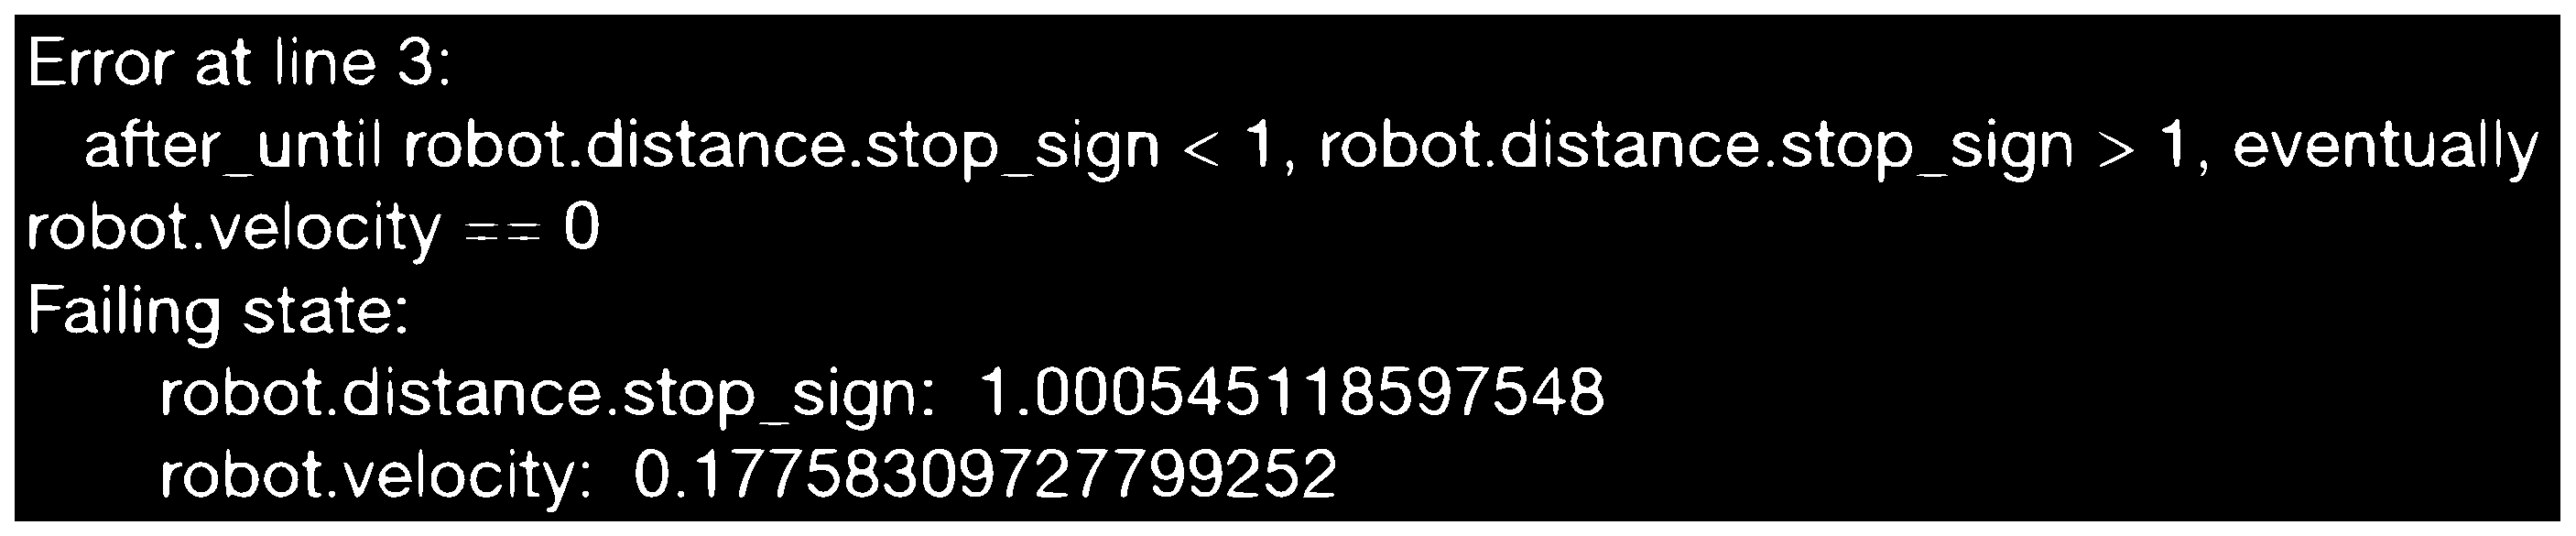
\includegraphics[width=\textwidth]{images/error.eps}
\caption{Example of the displayed error when the robot does not stop at the stop sign.} \label{fig:error}
\end{figure}

The flow of the process of monitoring a robotic system is described as follows:

\begin{enumerate}[label=(\roman*)]
    \item \textbf{Property formalization:} The developer describes in the DSL the properties of the robotic system one wants to monitor in a \texttt{.txt} file extension.
    \item \textbf{Compilation:} The specified properties are compiled, and a python file is generated capable of running as a ROS node.
    \item \textbf{Monitoring:} The node can be run whenever testing the system and will listen to pertinent topics and perform the computations needed to verify the specified properties.
\end{enumerate}


% ------------------------------------------------------------------------------
% Contributions
\section{Contributions}
\label{sec:contributions}

The expected contributions of this thesis are below enumerated.

\begin{enumerate}
    \item Definition of a domain-specific language to specify robotic systems' properties.
    \item Implementation of a compiler for the language that can generate software capable of monitoring relevant components while in a simulation.
    \item Evaluation of the expressive capabilities of the solution.
\end{enumerate}


% ------------------------------------------------------------------------------
% Structure of the document
\section{Structure of the document}
\label{sec:structure}

The document is organized as follows:

\begin{itemize}
    \item \autoref{chap:background} - Background \& Related Work:
    \item \autoref{chap:language} - Specification Language for Robotics Properties
    \item \autoref{chap:monitoring} - Monitoring
    \item \autoref{chap:evaluation} - Evaluation 
    \item \autoref{chap:futurework} - Future Work
    \item \autoref{chap:conclusion} - Conclusion
\end{itemize}

% !TeX root = ../main.tex
\chapter{Background \& Related Work}
\label{chap:background}

*Write structure after writing everything*

\section{Software}

*structure*

% ------------------------------------------------------------------------------
% ROS
\subsection{Robot Operating System}
\label{sec:ros}

The Robot Operating System (ROS)~\cite{quigley2009ros} is an open-source framework with a vast collection of libraries, interfaces, and tools that were designed to help build robot software. ROS provides an abstraction between hardware and software that helps developers easily connect the different robot components through messages sent through communication channels (\textit{topics}).

ROS has a modular architecture along with other advantages that were built with the purpose of cross-collaboration and easy development. For all these reasons ROS is used by hundreds of companies and research labs.

% ------------------------------------------------------------------------------
% Gazebo
\subsection{Gazebo}
\label{sec:gazebo}

Robotic systems simulation is an essential tool for testing robots' behavior, for this reason, Gazebo~\cite{koenig2004design} started with the idea of a high-fidelity simulator to simulate robots in any type of environment under mixed conditions.

Gazebo is an open-source 3D simulator that supports tools like sensors simulation, mesh management, and actuators control under different physics engines, among others, which makes it a simulator that can be used by very distinct robotic systems.

% ------------------------------------------------------------------------------
% Linear Temporal Logic
\section{Linear Temporal Logic}
\label{sec:ltl}

Linear temporal logic (LTL) is a branch of logic responsible for representing and reasoning about modalities in reference to time. 

As an approach for program verification, a formal system of temporal logic was suggested for both sequential and parallel programs~\cite{pnueli1977temporal}. LTL can be used as a method of model-checking~\cite{dwyer1998property} using its patterns as a form of property specification. It includes patterns such as "always", "finally", "until", "eventually", and others, which can be useful in the creation of invariants for program verification.

% ------------------------------------------------------------------------------
% Property Specification
\section{Robot Testing}
\label{sec:robottesting}

\subsection{Invariants}
%https://clairelegoues.com/papers/zizyte21dsn.pdf
%~\cite{zizyte2021importance}

\subsection{Runtime Monitoring}
%https://rose-workshops.github.io/files/rose2022/papers/RoSE22_paper_4.pdf
%~\cite{stadler2022towards}

\subsection{Similar work}
%ROSMonitoring~\cite{ferrando2020rosmonitoring}
%ROSRV~\cite{huang2014rosrv}

% !TeX root = ../main.tex
% %%%%%%%%%%%%%%%%%%%%%%%%%%%%%%%%%%%%%%%%%%%%%%%%%%%%%%%%%%%%%%%%%%%%%%%%%%%%%%
% Language
\chapter{Specification Language for Robotics Properties}
\label{chap:language}

In this chapter, the structure and intricacies of the DSL are presented. *Explain each section*

% ------------------------------------------------------------------------------
% High-Level Notations
\section{High Level Notations}

\begin{itemize}
\item \textbf{Property -} A property represents a temporal specification or a blend of temporal specifications between components.
\item \textbf{Declaration -} A declaration allows for the representation of ROS \textit{topics} in order to interact with it.
\item \textbf{Model -} A model allows for the declaration of specific \textit{topics} that are required when correlating certain robots' and simulation components.
\item \textbf{Association -} An association serves as a way to create program variables.
\end{itemize}

% ------------------------------------------------------------------------------
% Temporal Keywords
\subsection{Temporal Keywords}

We consider not only LTL basic operators but also some common shortcuts for useful combinations of such operators, like \textit{after\_until}.

\begin{itemize}
\item {\bfseries always X} - X has to hold on the entire subsequent path;
\item {\bfseries never X} - X never holds on the entire subsequent path;
\item {\bfseries eventually X} - X eventually has to hold somewhere on the subsequent path;
\item {\bfseries after X, Y} - after the event X is observed, Y has to hold on the entire subsequent path;
\item {\bfseries until X, Y} - X holds at the current or future position, and Y has to hold until that position. At that position, Y does not have to hold anymore;
\item {\bfseries after\_until X, Y, Z} - after the event X is observed, Z has to hold on the entire subsequent path up until Y happens. At that position, Z does not have to hold anymore;
\end{itemize}

%\noindent It is also possible to reference previous states of variables, using \textbf{\lstinline|@{X, -y}|}, representing the value of variable \lstinline|X| at time \lstinline|-y|.

% ------------------------------------------------------------------------------
% Temporal value
\subsection{Temporal value}

It is also possible to reference previous variable states:
\begin{equation}
@\{X, -y\}
\end{equation}
This will represent the value of the variable X in the point in time -y.

% ------------------------------------------------------------------------------
% Functions
\subsection{Simulation primivitives}

To support comparing the internal state of the robotic system with the environment, we provide basic primitives in the language to refer to the simulation environment:

\begin{itemize}
\item {\bfseries X.position} - The position of the robot in the simulation;
\item {\bfseries X.position.y} - The position in the y axis of the robot in the simulation. Also works for x and z;
\item {\bfseries X.distance.Y} - The absolute distance between two objects in the simulation. For the x and y axis;
\item {\bfseries X.distanceZ.Y} - The absolute distance between two objects in the simulation. For the x, y, and z axis;
\item {\bfseries X.velocity} - The velocity of an object in the simulation. This refers to linear velocity;
\item {\bfseries X.velocity.x} - The velocity in the x axis of an object in the simulation. This refers to linear velocity;
\item {\bfseries X.localization\_error} - The difference between the robot's perception of its position and the actual position in the simulation;
\end{itemize}

% ------------------------------------------------------------------------------
% Operands
\section{Operands}

Besides the already mentioned operands, \textit{Temporal values}, \textit{Simulation primivitives}, and \textit{Temporal Keywords}, the DSL also supports both Integer and Float values, Booleans, and declared variables.

% ------------------------------------------------------------------------------
% Operators
\section{Operators}

The DSL supports operators to correlate components. The operators are \textit{+} (addition), \textit{-} (subtraction), \textit{*} (multiplication), \textit{/} (division), \textit{==} (equals), \textit{!=} (different), \textit{>} (greater than), \textit{>=} (greater or equal than), \textit{<} (lower than), \textit{<=} (lower or equal than), \textit{and} (conjunction), \textit{or} (disjunction), \textit{implies} (implication), and for any comparison operator X \textit{X{y}} - the values being compared will have an error margin of y (Example: Z =={0.05} Y).

% ------------------------------------------------------------------------------
% Protected Variables
\section{Protected Variables}

Protected variables are variable names restricted to set determined monitoring parameters.

\_rate\_ - Set the frame rate which properties are checked (By default, the rate is 30hz)

\_timeout\_ - Set the timeout for how long the verification will last (By default, the timeout is 100 seconds)

\_margin\_ - Set the error margin for comparisons

% ------------------------------------------------------------------------------
% Topic declaration
\section{Topic declaration}

In order to relate robot components with the simulation, the developer can declare the relevant \textit{topics}.

The language cannot inherently have a way to interact with specific components of a robot because it does not know which topic to get information from. Therefore, the developer needs to declare these specific topics to be able to interact with them.

\textit{The variable robot\_position was declared with the type Odometry.pose.pose.position and is linked to the topic /odom;}

%\vspace{2mm}

\texttt{decl robot\_position /odom Odometry.pose.pose.position}

% ------------------------------------------------------------------------------
% Model robots
\section{Model robots}

A set of specific topics can be modeled for the robot, like \textit{position} or \textit{velocity}. The compiler will use these to call specific functions that need this information from the robot's perspective.

%\vspace{2mm}

\texttt{model robot1:}

\texttt{    position /odom Odometry.pose.pose.position}

\texttt{    ;}

%\vspace{2mm}

\texttt{never robot1.localization error > 0.002}

% ------------------------------------------------------------------------------
% Grammar
\section{Grammar}

\begin{bnfgrammar}
    <program> : Start
    ::=
    <command> || <command> <program>
    ;;
    <command> ::=
    <association>
    | <declaration>
    | <model>
    | <pattern>
    ;; 
    <association> ::=
    name = <pattern>
    | \_rate\_ = integer
    | \_timeout\_ = <number>
    | \_default\_margin\_ = <number>
    ;;
    <declaration> ::=
    decl name topic\_name <msgtype>
    | decl name name <msgtype>
    ;;
    <model> ::= 
    model name \: <modelargs> ; %TODO escape :
    ;;
    <modelargs> ::= 
    <name> topic\_name <msgtype>
    | <name> <name> <msgtype>
    | <name> topic\_name <msgtype> <modelargs>
    | <name> <name> <msgtype> <modelargs>
    ;;
    <name> ::= 
    name || <func\_main>
    ;;
    <func\_main> ::= 
    position
    | velocity
    | distance
    | localization\_error
    | orientation
    ;;
    <msgtype> ::= 
    <name> || <name> . <msgtype>
    ;;
    <pattern> ::= 
    always <pattern>
    | never <pattern>
    | eventually <pattern>
    | after <pattern> , <pattern>
    | until <pattern> , <pattern>
    | after\_until <pattern> , <pattern> , <pattern>
    | <conjunction>
    ;;
    <conjunction> ::= 
    <conjunction> and <comparison>
    | <conjunction> or <comparison>
    | <conjunction> implies <comparison>
    | <comparison>
    ;;
    <comparison> ::= 
    <multiplication> <opbin> <multiplication>
    | <multiplication> <opbin> { <number> } <multiplication>
    | <multiplication>
    ;;
    <opbin> ::= 
    < || > || <= || >= || == || !=
    ;;
    <multiplication> ::= 
    <multiplication> * <addition>
    | <multiplication> / <addition>
    | <addition>
    ;;
    <addition> ::= <addition> + <operand>
    | <addition> - <operand>
    | <operand>
    ;;
    <operand> ::= 
    name || <number> || true || false || <func> || <temporalvalue> || ( <pattern> )
    ;;
    <number> ::= 
    float || integer
    ;;
    <func> ::= 
    name . <func\_main>
    | name . <func\_main> <funcargs>
    ;;
    <funcargs> ::= 
    . <name> || . <name> <funcargs>
    ;;
    <temporalvalue> ::= 
    @ { name , integer }
\end{bnfgrammar}

% !TeX root = ../main.tex
% %%%%%%%%%%%%%%%%%%%%%%%%%%%%%%%%%%%%%%%%%%%%%%%%%%%%%%%%%%%%%%%%%%%%%%%%%%%%%%
% Monitoring
\chapter{Monitoring}
\label{chap:monitoring}

This chapter explains the whole process of monitoring, from compilation to error detection. First, the overall process of compilation is explained (\autoref{sec:runtimemonitoring}), then the generated file and some of its specifications are described (\autoref{sec:generatedfile}), and finally, the shown error messages are illustrated (\autoref{sec:errormessages}).


% ------------------------------------------------------------------------------
% Runtime Monitoring
\section{Runtime Monitoring}
\label{sec:runtimemonitoring}

After writing all the desired robotic systems specifications, the file needs to be compiled to generate the monitoring python file. Currently, to compile a specification file, one has to do it through the console under the same directory of the \textit{language.py} file. As for the command:

\texttt{python language.py properties.txt /home/ros\_workspace/src/my\_pkg/src}

The \textit{language.py} file needs to be run as a python file and be given as arguments:

\begin{enumerate}
    \item The specifications file name, and in case it is not in the same directory as the \textit{language.py} file, give its absolute path.
    \item The expected absolute path of the generated python monitoring file.
\end{enumerate}

The given directory for the generated file should be under a ROS workspace for the compilation to succeed. This is because, during the compilation, access to information like the available ROS messages might be necessary.

The monitoring file can now run as an independent ROS node, integrated into a launch file, or using rosrun in the console to execute it.


% ------------------------------------------------------------------------------
% Generated File
\section{Generated File}
\label{sec:generatedfile}

Declare the needed subscribers and use ApproximateTimeSynchronizer to call the callback function. The ApproximateTimeSynchronizer synchronizes messages by their timestamp and if they do not have a header, use the ROS time.

The callback function is called every time a new message from one of the subscribers is received. The callback function saves the relevant information for property checking in a global variable. This information serves as a current "screenshot" of the simulation representing its current state.

The node executes a loop at a delineated rate, doing the following tasks. 

Check if the defined simulation timeout time has reached. 

Save the current simulation state obtained by the callback function. This is necessary because the callback function is called at fluctuating rates, and we want to save multiple "screenshots" of the simulation at the loop fixed rate to make correlations with past states. 

Verify the properties using the saved states and calling each created function. An independent function with the necessary computations for verifying the property is defined for each base property.


% ------------------------------------------------------------------------------
% Error Messages
\section{Error Messages}
\label{sec:errormessages}

An error message starts by stating the line in the specification file which resulted in an error and showing the specification itself.

Afterward, the value at the time of failure of all the variables present at the specification is shown.

\begin{figure}[h]
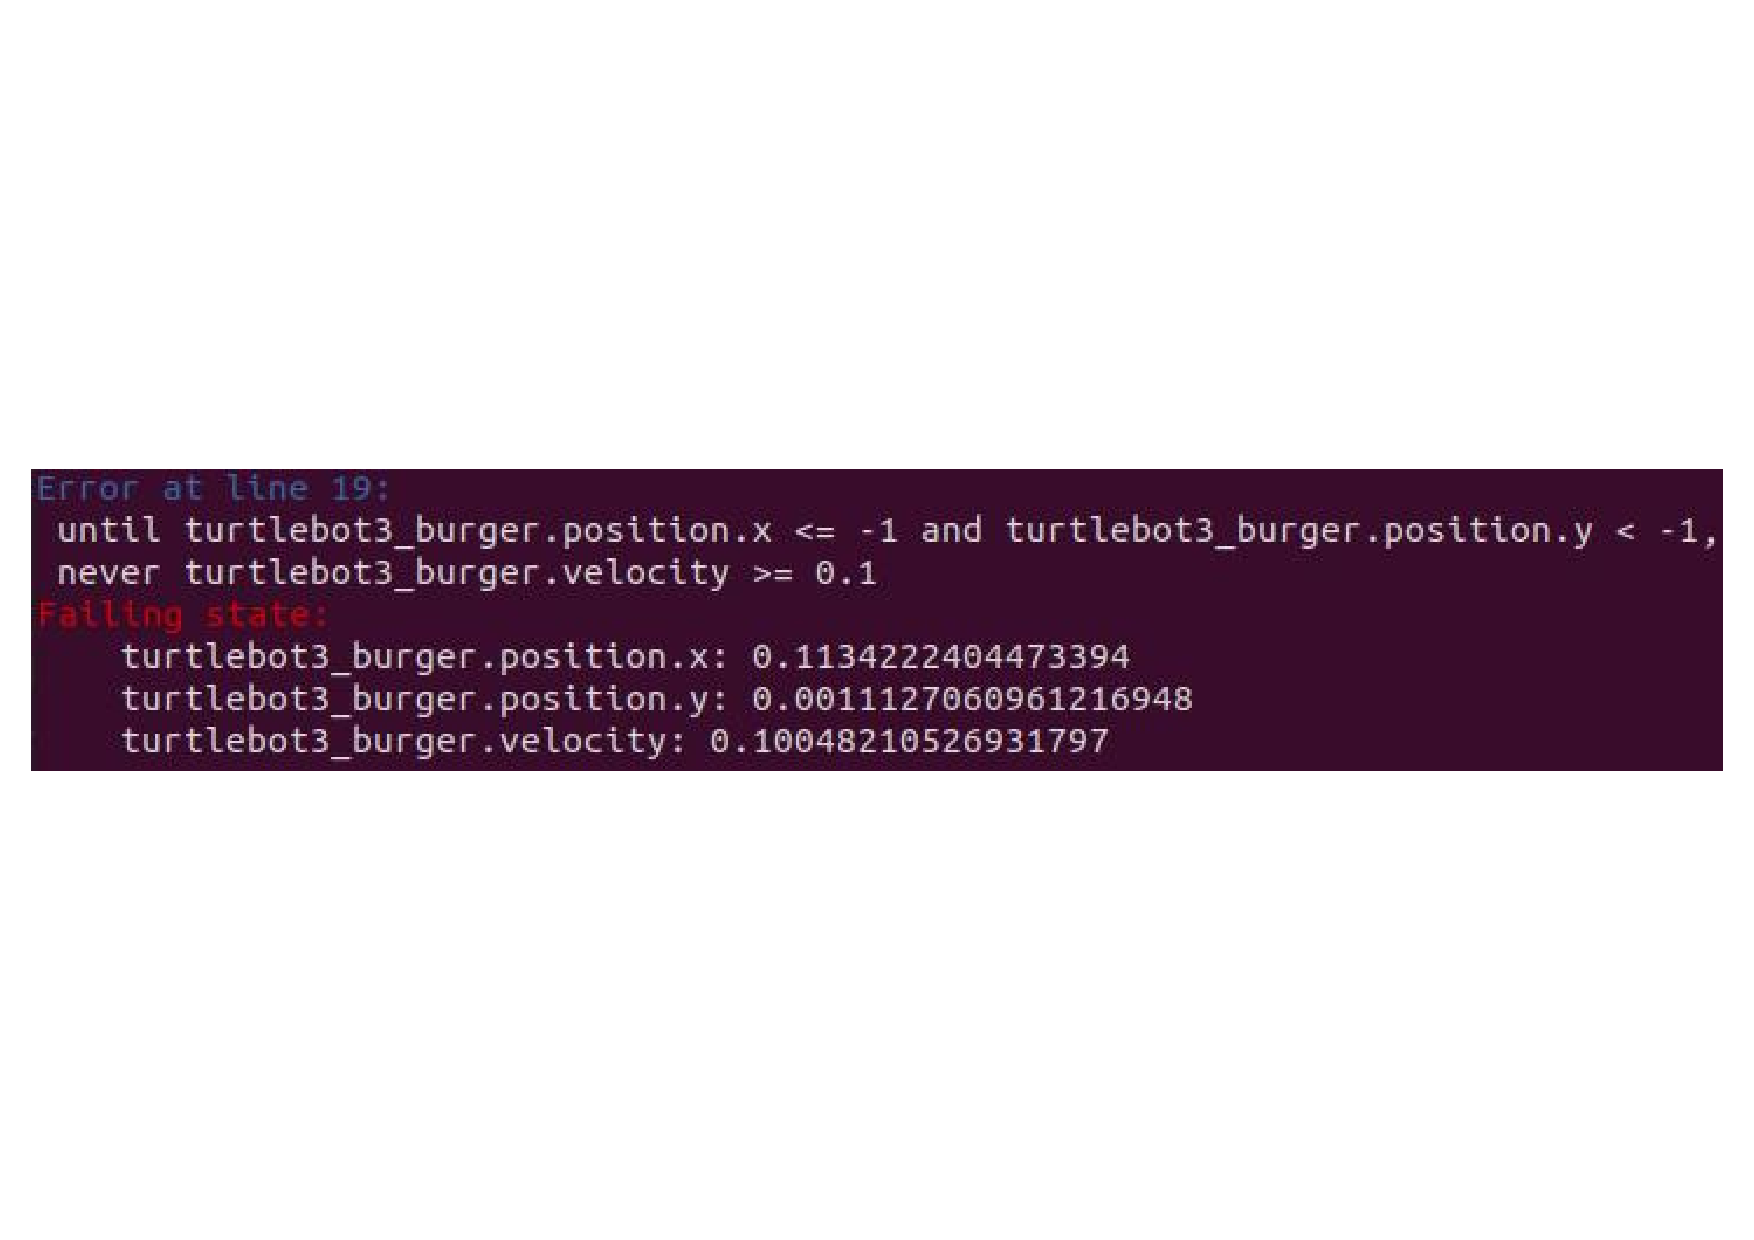
\includegraphics[width=\textwidth]{images/error_message.pdf}
\caption{Example of an error message.} \label{fig:monerror}
\end{figure}
% !TeX root = ../main.tex
% %%%%%%%%%%%%%%%%%%%%%%%%%%%%%%%%%%%%%%%%%%%%%%%%%%%%%%%%%%%%%%%%%%%%%%%%%%%%%%
% Evaluation
\chapter{Evaluation}
\label{chap:evaluation}

This chapter introduces the evaluation process of the work. \autoref{sec:evaluationoverview} gives a broad overview of the whole process, and \autoref{sec:experiments} goes into more detail about each one of the experiments.


% ------------------------------------------------------------------------------
% Evaluation Overview
\section{Evaluation Overview}
\label{sec:evaluationoverview}

To evaluate the developed work, I decided to go through a list of already documented ROS bugs and identify three that happen at runtime. After that, I specified a robot's properties in the DSL that should be capable of detecting an error for said bugs while running the system.

ROBUST~\cite{robust} is a dataset that documents over two hundred bugs in multiple robots using ROS. After going through the dataset, three bugs were chosen:

\begin{itemize}
    \item Calculation Error Inverts Turning Direction~\footnote{\url{https://github.com/robust-rosin/robust/blob/master/kobuki/e964bbb/e964bbb.bug}} (\autoref{ssec:calculationerrorinvertsturningdirection}) - "Due to an error in velocity calculations, when Kobuki was issued a very low negative linear speed (very slow backwards movement), it would also inadvertently invert its turning direction. That is, if it was supposed to move backwards while turning left, it would move backwards and turn right instead."
    \item Robot Getting Stuck When Auto-docking~\footnote{\url{https://github.com/robust-rosin/robust/blob/master/kobuki/0416c81/0416c81.bug}} (\autoref{ssec:robotgettingstuckwhenautodocking}) - "The movement speeds were hard-coded for the auto-docking algorithm, and worked well for regular Kobuki and Turtlebot, but were too slow for heavier robots, causing them to get stuck."
    \item Unexpected Movement Due to Wrong Calculation~\footnote{\url{https://github.com/robust-rosin/robust/blob/master/kobuki/1c141a5/1c141a5.bug}} (\autoref{ssec:unexpectedmovementduetowrongcalculation}) - "Kobuki moves using differential drive. Originally, the command velocities (linear and angular) were provided as `short`, and were converted to `short` after each step, even though the calculations yielded floating point numbers. This lead to calculation errors in some special cases, where the robot was supposed to move forward but ended up moving backwards instead."
\end{itemize}

To replicate each bug, a \textit{daemon} node is inserted into the system that interferes with the normal runtime flow and replicates the desired bug. \autoref{fig:normalflow} represents the natural flow of the systems whilst \autoref{fig:demonflow} shows the system flow when trying to replicate a bug with the help of the \textit{daemon} node.

\begin{figure}[htb]
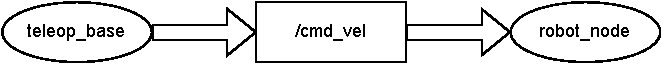
\includegraphics[width=\textwidth]{images/normal_flow.pdf}
\caption{The normal runtime flow of the system.} \label{fig:normalflow}
\end{figure}
    
\begin{figure}[htb]
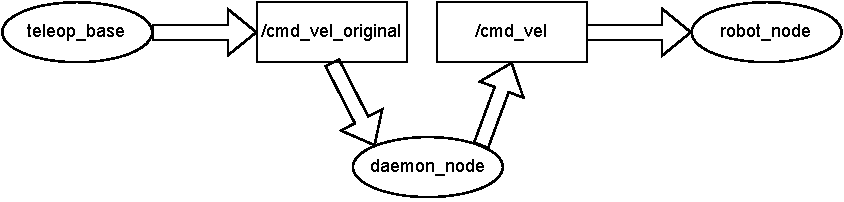
\includegraphics[width=\textwidth]{images/demon_flow.pdf}
\caption{The flow of the system when the adding the daemon node.} \label{fig:demonflow}
\end{figure}

When injecting a bug, all the data before addressed to the robots' \textit{/cmd\_vel} topic is remapped to a new topic called \textit{/cmd\_vel\_original}, the \textit{daemon} node subscribes to this new topic and modifies the data before sending it to the robots' \textit{/cmd\_vel} topic so that the robot behaves like the expected bug. 

With this new system flow, it is possible to specify properties between the \textit{/cmd\_vel} topic which represents the robots' behavior, and the \textit{/cmd\_vel\_original} topic, which represents the actual command given to the robot.


% ------------------------------------------------------------------------------
% Experiments
\section{Experiments}
\label{sec:experiments}

This section goes through the property specification and runtime monitoring for the three mentioned selected bugs. Calculation Error Inverts Turning Direction (\autoref{sec:background}), Robot Getting Stuck When Auto-docking(\autoref{sec:background}), and Unexpected Movement Due to Wrong Calculation (\autoref{sec:background}).


% ------------------------------------------------------------------------------
% Calculation Error Inverts Turning Direction
\subsection{Calculation Error Inverts Turning Direction}
\label{ssec:calculationerrorinvertsturningdirection}

DSL property specification:

First, I declare the cmd\_vel\_original topic, which will represent the commands given to the robot.
Then I make a correlation between the topic that represents the given commands and the topic that represents the actual robot's behavior.

\texttt{decl angular\_vel\_robot\_perception cmd\_vel\_original Twist.angular.z}

\texttt{after turtlebot3.velocity.angular.z < 0, never angular\_vel\_robot\_perception > 0}

\textit{Translating into natural language, the property states in the first section that after the robot's actual simulation z parameter of the angular velocity is less than zero, then in the second section, never the z parameter of the angular velocity of the command given to the robot is more than zero.}

\textit{Daemon} node code and behavior:

\begin{lstlisting}[language=Python]
    class Direction_invert_error:

        def __init__(self):
            print("simulating direction_invert_error_behavior...")
            self.cmd_vel_pub = rospy.Publisher("cmd_vel", Twist, queue_size=1)
            self.twist = Twist()
            self.direction_invert_error()

        def get_vel(self):
            return rospy.wait_for_message("cmd_vel_original", Twist)

        def direction_invert_error(self):
            while not rospy.is_shutdown():
                vel = self.get_vel()
                self.twist = vel
                if abs(vel.linear.x) < 0.012:
                    self.twist.angular.z = -vel.angular.z
                self.cmd_vel_pub.publish(self.twist)
\end{lstlisting}

The \textit{daemon} node checks when the given robot's command linear velocity is below \textit{0.012} and injects the opposite value of the z parameter of the angular velocity to the actual robot's velocity in the simulation.

Now when giving commands to the robot, if the given velocity is below \textit{0.012} and I make a turn, the robot will turn the opposite way. The output of the monitoring node for a test case is demonstrated in \autoref{fig:erreval1}.

\begin{figure}[htb]
\begin{center}
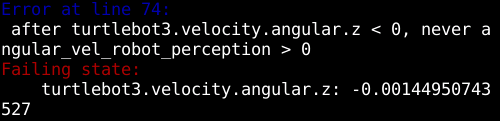
\includegraphics[width=8cm,height=2cm,keepaspectratio,]{images/erreval1.png}
\caption{Calculation Error Inverts Turning Direction bug error message.} \label{fig:erreval1}
\end{center}
\end{figure}


% ------------------------------------------------------------------------------
% Calculation Error Inverts Turning Direction
\subsection{Robot Getting Stuck When Auto-docking}
\label{ssec:robotgettingstuckwhenautodocking}

DSL property specification:

First, I declare the cmd\_vel\_original topic, which will represent the commands given to the robot.
Then I make a correlation between the topic that represents the given commands and the topic that represents the actual robot's behavior.

\texttt{decl vel\_robot\_perception cmd\_vel\_original Twist.linear.x}

\texttt{after vel\_robot\_perception > 0, never turtlebot3.velocity =={0.005} 0}

\textit{Translating into natural language, the property states in the first section that after the given robot's commands x parameter of the linear velocity is greater than zero, then in the second section never, the actual simulation's linear velocity is equal to zero.}

\textit{Daemon} node code and behavior:

\begin{lstlisting}[language=Python]
    class Auto_docking_error:

        def __init__(self):
            print("simulating auto_docking_error_behavior...")
            self.cmd_vel_pub = rospy.Publisher("cmd_vel", Twist, queue_size=1)
            self.twist = Twist()
            self.auto_docking_error()

        def get_vel(self):
            return rospy.wait_for_message("cmd_vel_original", Twist)

        def auto_docking_error(self):
            while not rospy.is_shutdown():
                vel = self.get_vel()
                self.twist = vel
                if abs(vel.linear.x) < 0.015:
                    self.twist.linear.x = 0.0
                self.cmd_vel_pub.publish(self.twist)
\end{lstlisting}

The \textit{daemon} node checks when the given robot's command linear velocity is below \textit{0.015} and injects a value of \textit{0.0} to the linear velocity of the actual robot's velocity in the simulation.

Now when giving commands to the robot, if the given velocity is below \textit{0.015} the robot will stay stationary. The output of the monitoring node for a test case is demonstrated in \autoref{fig:erreval2}.

\begin{figure}[htb]
\begin{center}
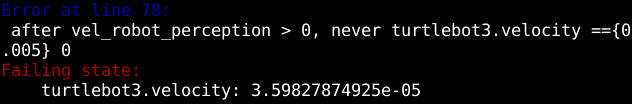
\includegraphics[width=10cm,height=3cm,keepaspectratio,]{images/erreval2.png}
\caption{Robot Getting Stuck When Auto-docking bug error message.} \label{fig:erreval2}
\end{center}
\end{figure}


% ------------------------------------------------------------------------------
% Calculation Error Inverts Turning Direction
\subsection{Unexpected Movement Due to Wrong Calculation}
\label{ssec:unexpectedmovementduetowrongcalculation}

DSL property specification:

First, I declare the cmd\_vel\_original topic, which will represent the commands given to the robot.
Then I make a correlation between the topic that represents the given commands and the topic that represents the actual robot's behavior.

\texttt{decl vel\_robot\_perception cmd\_vel\_original Twist.linear.x}

\texttt{after turtlebot3.velocity.linear.x < 0, never vel\_robot\_perception > 0}

\textit{Translating into natural language, the property states in the first section that after the robot's actual simulation x parameter of the linear velocity is less than zero, then in the second section, never the x parameter of the linear velocity of the command given to the robot is more than zero.}

\textit{Daemon} node code and behavior:

\begin{lstlisting}[language=Python]
    class Backwards_movement_error:

        def __init__(self):
            print("simulating backwards_movement_error_behavior...")
            self.cmd_vel_pub = rospy.Publisher("cmd_vel", Twist, queue_size=1)
            self.twist = Twist()
            self.backwards_movement_error()

        def get_vel(self):
            return rospy.wait_for_message("cmd_vel_original", Twist)

        def backwards_movement_error(self):
            while not rospy.is_shutdown():
                vel = self.get_vel()
                self.twist = vel
                if abs(vel.linear.x) > 0.03:
                    self.twist.linear.x = -vel.linear.x
                self.cmd_vel_pub.publish(self.twist)
\end{lstlisting}

The \textit{daemon} node checks when the given robot's command linear velocity is above \textit{0.03} and injects the opposite value of the x parameter of the linear velocity to the actual robot's velocity in the simulation.

Now when giving commands to the robot, if the given velocity is above \textit{0.03}, the robot will start moving backward. The output of the monitoring node for a test case is demonstrated in \autoref{fig:erreval3}.

\begin{figure}[htb]
\begin{center}
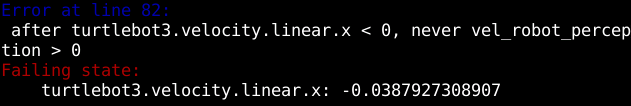
\includegraphics[width=10cm,height=3cm,keepaspectratio,]{images/erreval3.png}
\caption{Unexpected Movement Due to Wrong Calculation bug error message.} \label{fig:erreval3}
\end{center}
\end{figure}

%\todo{Feels like it's missing a section with a list of real-world bugs that could be detected with your language, even if you did not implement them.}

% !TeX root = ../main.tex
\chapter{Future Work}
\label{chap:futurework}

In this chapter the possible work left undone or that could improve our study is presented.
Improvement of the developed work performance is mentioned in \autoref{sec:performancetweaking}, \autoref{sec:validationproposal} mentions the validation of the work, \autoref{sec:bettererrormsg} discusses about the works' error messages, \autoref{sec:integratescenario} talks about the integration with scenario generation tools, and finally \autoref{sec:integratesimulators} mentions the possible integration with other simulators besides Gazebo.


% ------------------------------------------------------------------------------
% Performance Tweaking
\section{Performance Tweaking}
\label{sec:performancetweaking}

The generated code performance can be improved so that the load of the monitoring node on the simulation is reduced.

For instance, the frequency at which some properties are checked could fluctuate. In some circumstances, a particular property does not need to be checked at every simulation iteration. Implementing some mechanism that can skip certain property checks per iteration will undoubtedly decrease the load the monitoring node will have on the simulation.


% ------------------------------------------------------------------------------
% Validation of the Proposal
\section{Validation of the Proposal}
\label{sec:validationproposal}

Although some evaluation was done for the work done, more evidence and experimental data on the effective capabilities of the proposal are still needed:

\begin{enumerate}
    \item How expressive is the DSL from the developers' point of view in specifying robots' properties.
    \item Proof of concept that the system is able to detect the rule violations specified by the DSL.
    \item Evidence that the monitoring does not disturb the simulation by demanding excessive resources.
\end{enumerate}


% ------------------------------------------------------------------------------
% Better Error Messages
\section{Better Error Messages}
\label{sec:bettererrormsg}

Giving developers helpful and comprehensible error messages is a shared concern amongst all compilers. One can argue that even the best compilers still have space for improvement when talking about delivering good error messages.

Although in our work I gave some thought to the error messages delivery, I believe that a more narrow error localization is still possible.

Also, there was no time for a thorough validation of the proposal, which means that some bugs could be present when delivering the error messages, and the users could have some problems with the delivery or ideas on how to improve it.


% ------------------------------------------------------------------------------
% Integrate the DSL with Scenario Generation Tools
\section{Integrate the DSL with Scenario Generation Tools}
\label{sec:integratescenario}

Integrating our work with a scenario generation tool would improve the whole test automation process by creating unpredictable environments on where to test our specified properties, allowing the execution of multiple tests.

For instance, GzScenic~\cite{AfzalGzScenic} is a tool that generates random scenarios for the Gazebo simulator based on a defined model.


% ------------------------------------------------------------------------------
% Integration with other Industrial Simulators
\section{Integration with other Industrial Simulators}
\label{sec:integratesimulators}

Our work was developed with the Gazebo simulator in mind, which means the monitoring is currently not compatible with other simulators.

Although Gazebo is widely used, many other simulators are also currently being used. Therefore, adapting our work to integrate other widely used simulators would be helpful for many users that choose not to use Gazebo.

\todo{What other simulators are there?}


%Worth mentioning? - The tests could allow the robot's automatic correction and generation of code. Generating multiple alternatives and automatically evaluating how good they are, improving the code to do what we want.*

\todo{This work can be used to measure quality of software modules. thus, it can be used in automated program synthesis, repair and improvement}

% !TeX root = ../main.tex
\chapter{Conclusion}
\label{chap:conclusion}


Due to the fact that robots interact with the real world, robotic systems are unpredictable. Coming up with a reliable and efficient method for automatic robot testing is a challenge, one of the reasons being that verifying the success of a task may not be possible from the robot's perspective. Current practices in testing robot software mainly require a human to analyze the robot's behavior to determine its correctness, one way of overcoming this problem is with some other type of automatic external monitoring.

Our approach relies on simulation-based testing so that developers can take advantage of the real values of objects'
attributes on the simulation to compare with what the robot system perceives, trying in this way to surpass the need for human-in-the-loop testing.

We developed a DSL that allows for the specification of a robotic system's properties, designed from the ROS framework point of view, and that abstracts the underlying LTL system. As a result, it is possible to express relevant temporal and positional arguments between robots' components and objects in the simulation and also properties that relate the internal information of the system with the corresponding information in the Gazebo simulator.

We automated the generation of a monitoring python file that can monitor some behavioral violations of robots in relation to their state or events during a Gazebo simulation.

We have shown that the approach can monitor some interesting scenarios that developers care about. We also present what is still left to do and what future work is still needed.



% Appendixes
\appendix
% !TeX root = ../main.tex
% %%%%%%%%%%%%%%%%%%%%%%%%%%%%%%%%%%%%%%%%%%%%%%%%%%%%%%%%%%%%%%%%%%%%%%%%%%%%%%
% Appendixes
\chapter*{Appendix A}
\label{app:appendix-A}

\section{Displayed Error messages}

\begin{figure}
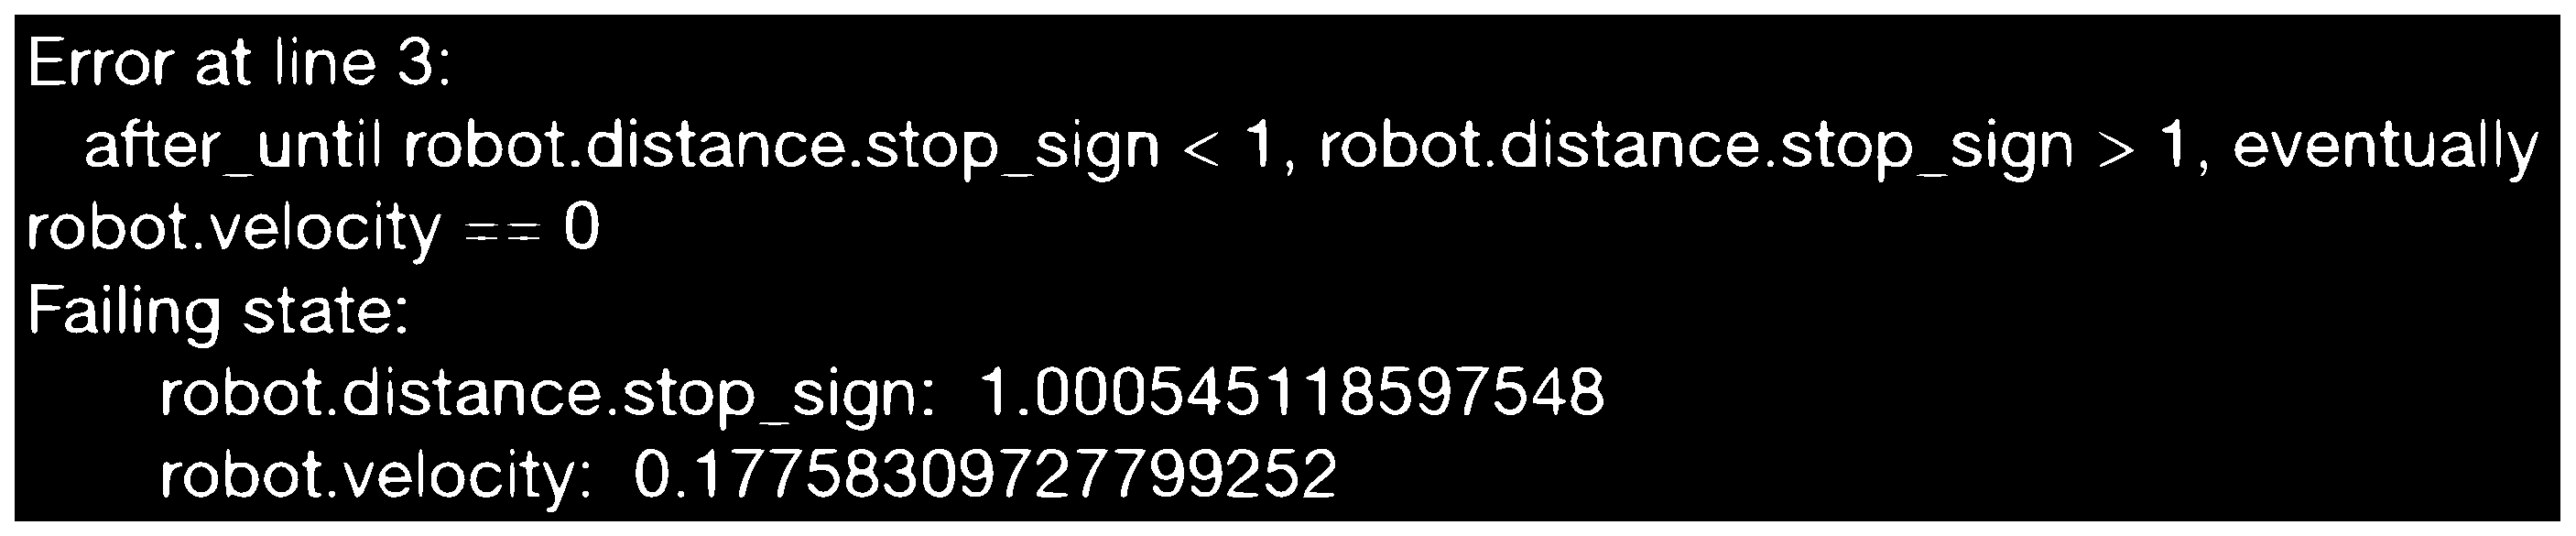
\includegraphics[width=\textwidth]{images/error.eps}
\caption{Example of the displayed error when the robot does not stop at the stop sign.}
\end{figure}

\begin{figure}[h]
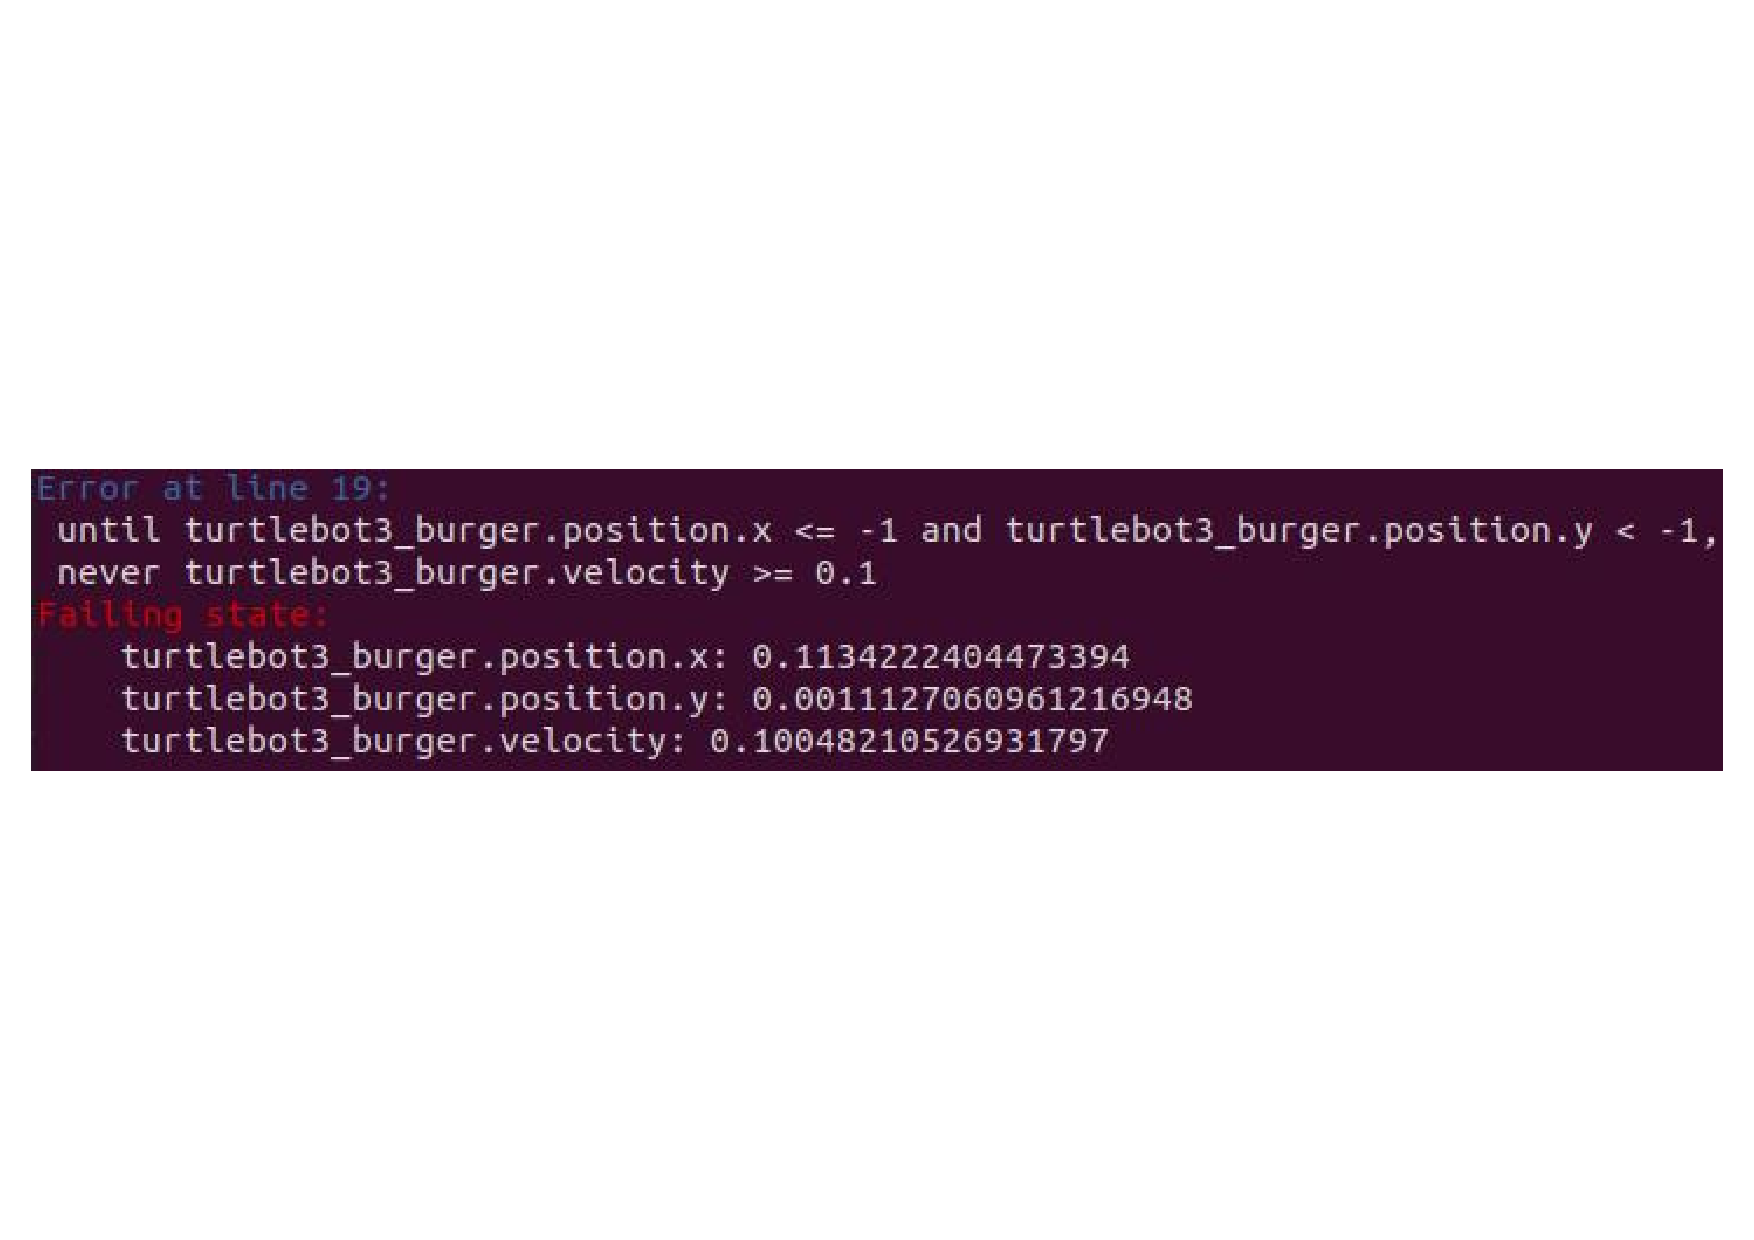
\includegraphics[width=\textwidth]{images/error_message.pdf}
\caption{Example of an error message.}
\end{figure}

\begin{figure}
\begin{center}
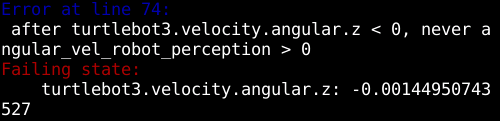
\includegraphics[width=8cm,height=2cm,keepaspectratio,]{images/erreval1.png}
\caption{Calculation Error Inverts Turning Direction bug error message.}
\end{center}
\end{figure}

\begin{figure}
\begin{center}
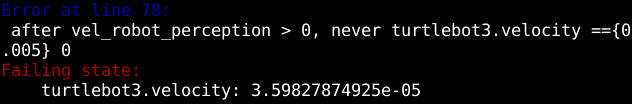
\includegraphics[width=10cm,height=3cm,keepaspectratio,]{images/erreval2.png}
\caption{Robot Getting Stuck When Auto-docking bug error message.}
\end{center}
\end{figure}

\begin{figure}
\begin{center}
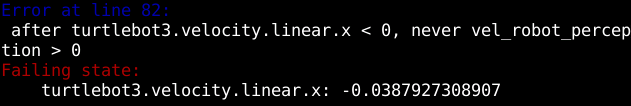
\includegraphics[width=10cm,height=3cm,keepaspectratio,]{images/erreval3.png}
\caption{Unexpected Movement Due to Wrong Calculation bug error message.}
\end{center}
\end{figure}


\chapter*{Appendix B}
\label{app:appendix-B}

\section{Evaluation Flow Diagrams}

\begin{figure}
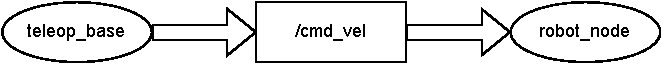
\includegraphics[width=\textwidth]{images/normal_flow.pdf}
\caption{The normal runtime flow of the system.}
\end{figure}
       
\begin{figure}
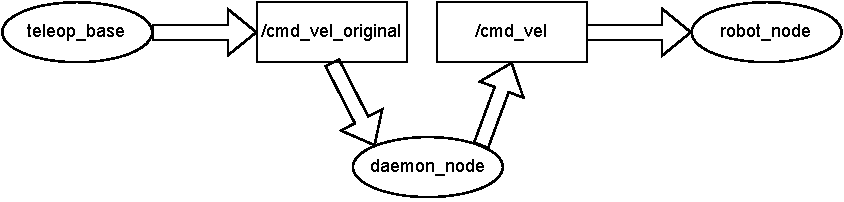
\includegraphics[width=\textwidth]{images/demon_flow.pdf}
\caption{The flow of the system when the adding the demon node.}
\end{figure}


% Bibliography
\bibliography{references}
\addcontentsline{toc}{chapter}{References}

\end{document}